\documentclass{./tufte-handout}

\usepackage{placeins}
\usepackage{caption}
\usepackage{subcaption}


\usepackage{amsmath, amssymb}

\usepackage{graphicx}
\setkeys{Gin}{width=\linewidth,totalheight=\textheight,keepaspectratio}
\graphicspath{{graphics/}}

\title{Statistical Machine Learning}
\author[Aakarsh Nair]{Aakarsh Nair\\aakarsh.nair@student.uni-tuebingen.de  \\Matriculation Number :6546577 }
\date{Due: 5 June 2024} 

% The following package makes prettier tables.  We're all about the bling!
\usepackage{booktabs}

% The units package provides nice, non-stacked fractions and better spacing
% for units.
\usepackage{units}

% The fancyvrb package lets us customize the formatting of verbatim
% environments.  We use a slightly smaller font.
\usepackage{fancyvrb}
\fvset{fontsize=\normalsize}

% Small sections of multiple columns
\usepackage{multicol}

% Provides paragraphs of dummy text
\usepackage{lipsum}

% These commands are used to pretty-print LaTeX commands
\newcommand{\doccmd}[1]{\texttt{\textbackslash#1}}% command name -- adds backslash automatically
\newcommand{\docopt}[1]{\ensuremath{\langle}\textrm{\textit{#1}}\ensuremath{\rangle}}% optional command argument
\newcommand{\docarg}[1]{\textrm{\textit{#1}}}% (required) command argument
\newenvironment{docspec}{\begin{quote}\noindent}{\end{quote}}% command specification environment
\newcommand{\docenv}[1]{\textsf{#1}}% environment name
\newcommand{\docpkg}[1]{\texttt{#1}}% package name
\newcommand{\doccls}[1]{\texttt{#1}}% document class name
\newcommand{\docclsopt}[1]{\texttt{#1}}% document class option name


\begin{document}

\maketitle

\section{Exercise 1: Ridge Regression}

\begin{enumerate}[(a)]
\item \textbf{(2 points)} In the following you have to implement least squares and ridge regression (both L2-loss)

\begin{itemize}
    \item \textbf{w = LeastSquares(Designmatrix,Y)}:
    \begin{itemize}
    \item  input: design matrix $\Phi \in R^{n  \times d}$ and the outputs $Y \in \mathbb{R}^n$ (column vector)
    \item output: weight vector w of least squares regression as column vector
    \end{itemize}

	\textbf{Answer:}
	See \emph{ridge.py} function \emph{ LeastSquares}. 
	
    \item  \textbf{w = RidgeRegression(Designmatrix,Y,Lambda)}:
    \begin{itemize}
        \item input: the design matrix $\Phi \in \mathbb{R}^n \times d$, the outputs 
        $Y \in \mathbb{R}^n$ (column vector), and the regularization
        parameter $\lambda \in \mathbb{R}^+ := \{x \in \mathbb{R}|x \geq 0\}$.
        \item output: weight vector w of ridge regression as column vector. Use the non-normalized version
        $w = {(\phi^T \phi + \lambda \mathbb{1}_d)}^{-1}\phi^T Y$ 
    \end{itemize}

       Note that that the regression with L1-loss is already provided in 
    \textbf{L1LossRegression(Designmatrix,Y,Lambda)}\\
    
    \textbf{Answer:} \\
    See \emph{ridge.py} function \emph{ RidgeRegression}. 
    
 
\end{itemize}



\item  \textbf{(1 points)} Let us assume that $d =1$. Write a function Basis(X, k) to generate the design matrix using 
the orthogonal Fourier basis functions, with
\begin{itemize}
    \item input: the input data matrix $X \in \mathbb{R}^{n \times 1}$ and 
    the maximal frequency $k$ of the Fourier basis. 
    \item output: the design matrix $\phi \in \mathbb{R}^{n \times (2k+1)}$  
    using the Fourier basis functions: 
    $\phi_{i,0} = 1$ for all $i = 1, . . . , n$ and 
    $\phi_{i,2l-1} = \cos(2\pi l x_i)$ and 
    $\phi_{i,2l} = \sin(2\pi l x_i)$ for all 
    $i = 1, . . . , n$ and $l = 1, . . . , k$.
\end{itemize}

\textbf{Answer:}\\

See \emph{ridge.py} function \emph{ Basis}. 


\item  In the first example we have only one feature $(d = )$ and thus we want to learn the function $f: \mathbb{R} \to \mathbb{R}$.  The data is given in \textbf{onedim.data.py} containing $Xtrain, Xtest, Ytrain, Ytest \in \mathbb{R}^{1000 \times 1}$.  First Plot the training data ${(Xtrain, Ytrain)}_{i=1}^{1000}$.

\begin{enumerate}
    \item \textbf{(1 Points)} Which loss functino ($L_1$ or $L_2$) is more appropriate for this
   kind of data? Justify this by checking the data plot.  Use in the next part only the regression method
   which your chosen loss (that is either regression or $L_1-loss$ with $L_2-regularizer$).

    \textbf{Answer:} \\
    We find that the ridge regression introduces a consistent bias  
    towards the outliers in the data for  all our plots for different 
    values of $k$. Thus in order to avoid this we use the \emph{L1LossRegression} 
    which is less biased towards the outliers.

    \begin{figure}[!ht]
        \centering
        \begin{subfigure}[b]{.5\textwidth}
          \centering
          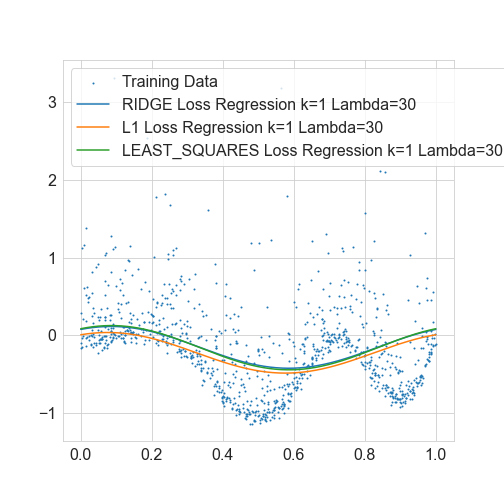
\includegraphics[width=1.2\linewidth]{../figures/l1_vs_ridge_regression_vs_least_squares_k_1_lambda_30.png}
          \caption{$k=1$}
        \end{subfigure}%
        \hfill
        \begin{subfigure}[b]{.5\textwidth}
          \centering
          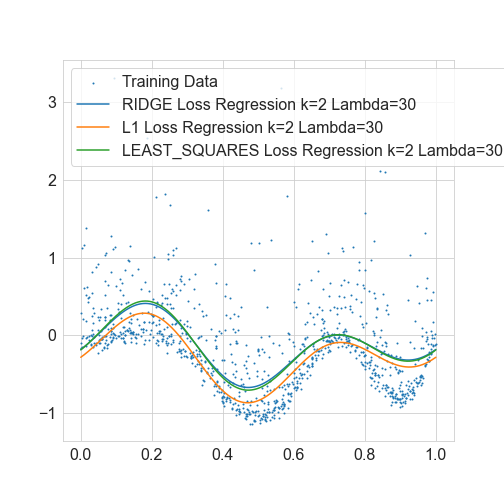
\includegraphics[width=1.2\linewidth]{../figures/l1_vs_ridge_regression_vs_least_squares_k_2_lambda_30.png}
          \caption{$k=2$}
        \end{subfigure}
        \begin{subfigure}[b]{.5\textwidth}
          \centering
          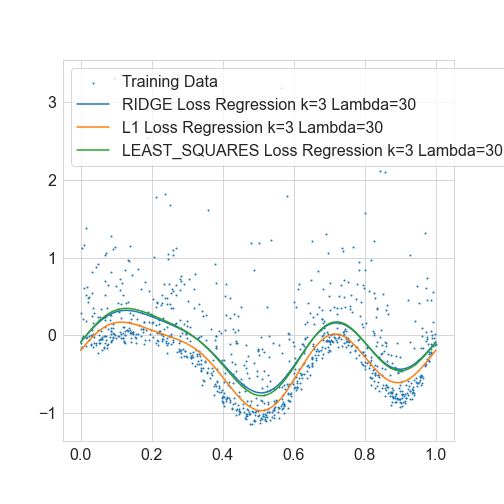
\includegraphics[width=1.2\linewidth]{../figures/l1_vs_ridge_regression_vs_least_squares_k_3_lambda_30.png}
          \caption{$k=3$}
        \end{subfigure}%
        \hfill
        \begin{subfigure}[b]{.5\textwidth}
          \centering
          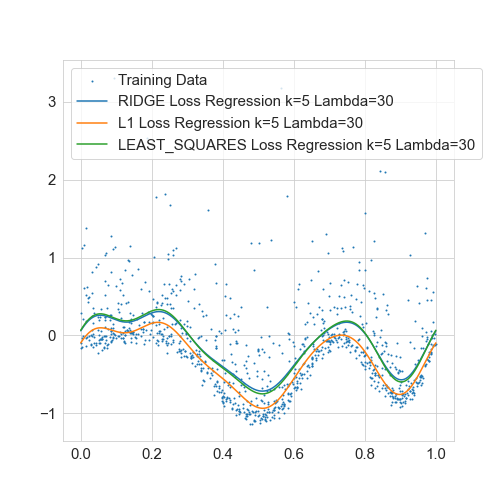
\includegraphics[width=1.2\linewidth]{../figures/l1_vs_ridge_regression_vs_least_squares_k_5_lambda_30.png}
          \caption{$k=5$}
        \end{subfigure}
        \begin{subfigure}[b]{.5\textwidth}
          \centering
          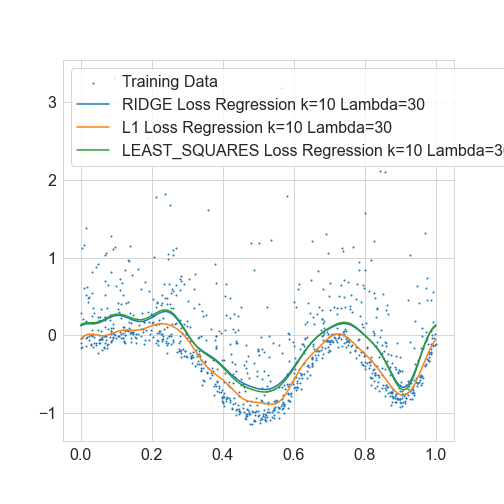
\includegraphics[width=1.2\linewidth]{../figures/l1_vs_ridge_regression_vs_least_squares_k_10_lambda_30.png}
          \caption{$k=10$}
        \end{subfigure}%
        \hfill
        \begin{subfigure}[b]{.5\textwidth}
          \centering
          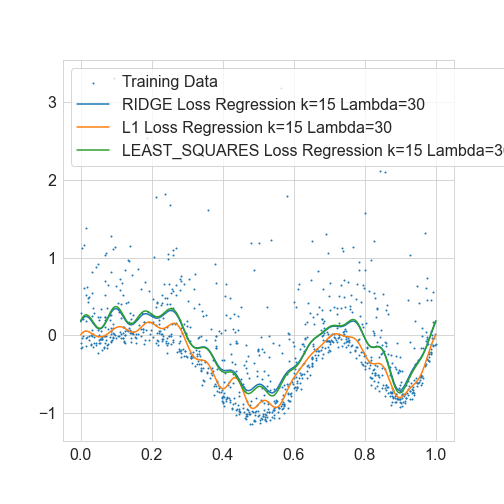
\includegraphics[width=1.2\linewidth]{../figures/l1_vs_ridge_regression_vs_least_squares_k_15_lambda_30.png}
          \caption{$k=15$}
        \end{subfigure}
        \hfill
        \caption{Comparison of L1,  Ridge Regression, Least Squares for different values of $k=1,2,3,5,10,15$. We note 
        that that ridge regression introduces a bias towards the outliers in the data}
    \end{figure}
    \FloatBarrier
    \item \textbf{(1 Points)} Use the basis function with $k=1, 2, 3, 5, 10, 15, 20$ from part b. to 
   to fit the regularized version of the loss chosen in the previous part. Use regularization paramater 
   $\lambda = 30$. Plot the resulting function $f_k$ (using as $x$ e.g 1000 evenly spaced points in $[0, 1]$) 
   for all values of $k$ together with the training data with: 

   \begin{equation}
        f_k(x)  = \langle \phi(x), w_k \rangle = \sum_{i=1}^{2k+1} w_i^k \phi_{i}(x)
   \end{equation}

   Compute the loss, that is 

   \begin{equation}
    \frac{1}{n}  \sum_{i=1}^n L(Y_i, f(X_i))
   \end{equation}

   on the training and test data and plot training and test loss as a function of $k$.
   Repeat the same for $\lambda =0$ (unregularized version). How does increasing 
   $k$ affect the estimated function $f_k$ ? 

   What is the behavior of training and test error for increasing 
   $k$ (explanation on paper). 

   \textbf{Answer:} \\

   We note that increasing the value of $k$ increases the function expressivity it 
   becomes rougher and begins to overfit to training data. This can be seen in 
   the loss curves, where th test loss fails to go down after $k=5$ while the training
   loss continues to decrease. This effect is more pronounced without regularization. 
   Where we note the curve for non-regularized Train loss has lowest value as $k$ 
   increases.
   
   \begin{figure}
    \centering
    \begin{subfigure}[b]{.5\textwidth}
        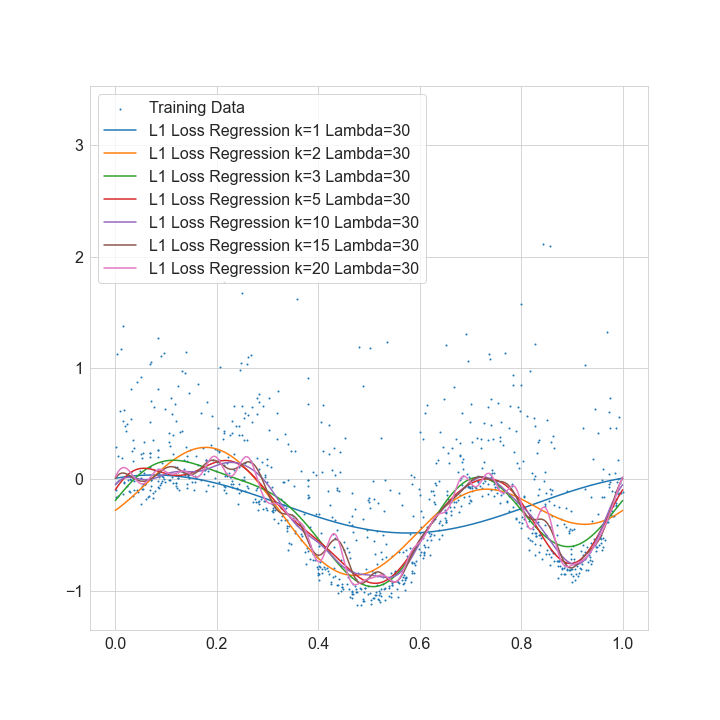
\includegraphics{../figures/l1_regression_all_k_lambda_30.png}
        \caption{L1 Loss Regression for all $k$ and $\lambda=30$.}
    \end{subfigure}%
    \begin{subfigure}[b]{.5\textwidth}
        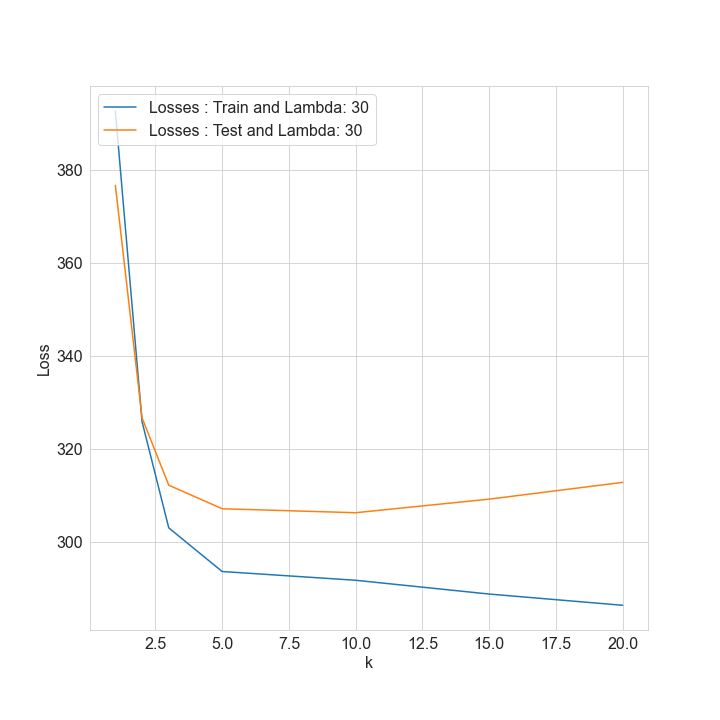
\includegraphics{../figures/l1_losses_for_k_lambda_30.png}
        \caption{Training and Test Loss for L1 Loss Regression and $\lambda=30$}
    \end{subfigure}
    \begin{subfigure}[b]{.5\textwidth}
        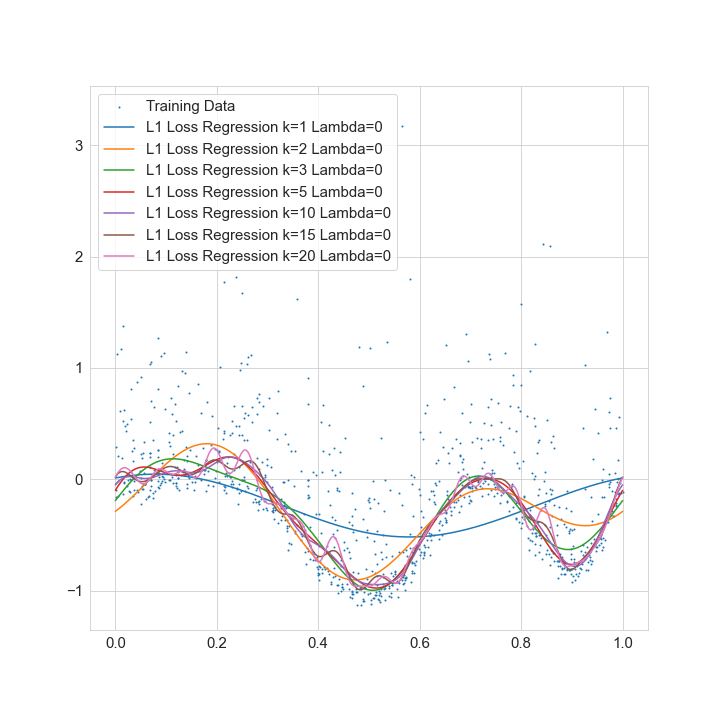
\includegraphics{../figures/l1_regression_all_k_lambda_0.png}
        \caption{L1 Loss Regression for all $k$ and $\lambda=0$.}
    \end{subfigure}%
    \begin{subfigure}[b]{.5\textwidth}
        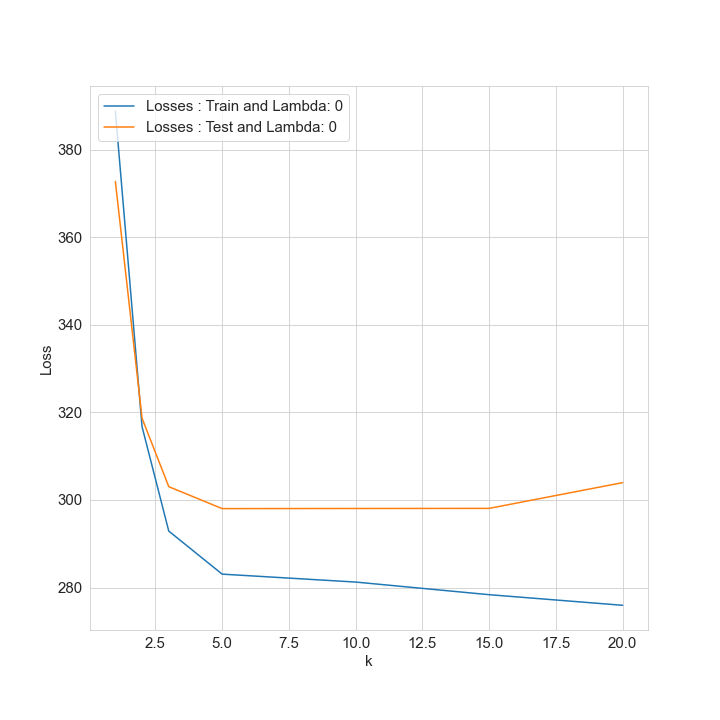
\includegraphics{../figures/l1_losses_for_k_lambda_0.png}
        \caption{Training and Test Loss for L1 Loss Regression and $\lambda=0$}
    \end{subfigure}

    \caption{Note that Test loss stabilizes around k=5 
    and increases subsequently, while training loss continues to decrease. 
    We note that $\lambda$=30 registers a higher training  loss than $\lambda$=0 as 
    regularization slows down overfitting to training data.}
   \end{figure}
   \FloatBarrier
\end{enumerate}
\FloatBarrier

\item On observes overfitting when we use large number $k$ of basis functions. We 
want to avoid this phenomenon by introducing a normalization of the basis functions according 
to their complexity. One possible way to do this is to define a measure of complexity $\Omega(f) \in \mathbb{R}^+$ as

\begin{equation}
    \Omega(f) = \int_0^1 |f'(x)|^2  dx
\end{equation}

where $f'$ is the first derivative of $f$ at x and introduce new Fourier basis functions $\{\Psi_i(x)\}_{i \in \mathbb{N}^0}$ as
\begin{equation}
    \Psi_0(x) = \Phi_0(x) 
\end{equation} 
and 
\begin{equation}
    \Psi_i(x) = \frac{1}{\sqrt{\Omega(\phi_i)}} \Phi_i(x) 
\end{equation}

$i \in \mathbb{N}^+$ where $\mathbb{N}^0 :=\{0, 1,2, \dots \}$ and 
\begin{enumerate}
    \item \textbf{(1 point)} Show the new Fourier basis functions $\Psi = {\Psi_i}_{ i\in \mathbb{N}^+}$ all have the same 
    complexity $\Omega(\Psi_i)$. 

    \textbf{Answer:}

    Consider 
    \begin{align} 
        \Omega(\Phi_i) &= \int_0^1 |(\Phi_i)'(x)|^2 dx
    \end{align}

    We know consider the case where $i=2l-1$ and $i=2l$ for $l \in [1..k]$. 

    \begin{align}
        \Omega(\Phi_{i=2l-1}) &= \int_0^1 |(\Phi_i)'(x)|^2 dx \\
            &= \int_0^1 | (\cos(2 \pi l x ))' |^2 dx \\
            &= \int_0^1 | -2 \pi l \sin(2 \pi l x) |^2 dx \\
            &= \int_0^1 (4 \pi^2 l^2) \sin^2(2 \pi l x) dx \\
            &= (4 \pi^2 l^2) \int_0^1  \sin^2(2 \pi l x) dx \\
            &= (4 \pi^2 l^2) \int_0^1  \frac{1 - \cos(4 \pi l x)}{2} dx \\
            &= (2 \pi^2 l^2) \int_0^1  1 - \cos(4 \pi l x) dx \\
            &= (2 \pi^2 l^2) \left[ x - \frac{1}{4 \pi l} \sin(4 \pi l x) \right]_0^1 \\
            &= (2 \pi^2 l^2) \left[ 1 - 0 - 0 + 0 \right] \\
            &= 2 \pi^2 l^2\\
        \sqrt{\Omega(\Phi_{i=2l-1})} &= \sqrt{2 \pi^2 l^2} \\
            &= \sqrt{2} \pi l
    \end{align}

    Now consider : 
    \begin{align}
        \Omega(\Phi_{i=2l}) &= \int_0^1 |(\Phi_i)'(x)|^2 dx \\
            &= \int_0^1 | (\sin(2 \pi l x ))' |^2 dx \\
            &= \int_0^1 | 2 \pi l \cos(2 \pi l x) |^2 dx \\
            &= \int_0^1 (4 \pi^2 l^2) \cos^2(2 \pi l x) dx \\
            &= (4 \pi^2 l^2) \int_0^1  \cos^2(2 \pi l x) dx \\
            &= (4 \pi^2 l^2) \int_0^1  \frac{1 + \cos(4 \pi l x)}{2} dx \\
            &= (2 \pi^2 l^2) \int_0^1  1 + \cos(4 \pi l x) dx \\
            &= (2 \pi^2 l^2) \left[ x + \frac{1}{4 \pi l} \sin(4 \pi l x) \right]_0^1 \\
            &= (2 \pi^2 l^2) \left[ 1 + 0 - 0 + 0 \right] \\
            &= 2 \pi^2 l^2\\
        \sqrt{\Omega(\Phi_{i=2l})} &= \sqrt{2 \pi^2 l^2} \\
            &= \sqrt{2} \pi l
    \end{align} 

    Thus the normalization constant is the same for both basis functions.

    Now we consider the complexity of the new basis functions $\Psi_i$:
    \begin{align}
            \Omega(\Psi_{i=2l-1}) &= \int_0^1 |(\Psi_i)'(x)|^2 dx \\
             &= \int_0^1 | \frac{1}{\sqrt{\Omega(\Phi_{i=2l-1})}} (\Phi_{i=2l-1})'(x) |^2 dx \\
             &= \int_0^1 | \frac{1}{\sqrt{2} \pi l} (-2 \pi l \sin(2 \pi l x)) |^2 dx \\
             &= \int_0^1 | \sqrt{2} \sin(2 \pi l x) |^2 dx \\
             &= \int_0^1 2 \sin^2(2 \pi l x) dx \\
             &= 2 \int_0^1 \frac{1 - \cos(4 \pi l x)}{2} dx \\
             &= \int_0^1 1 - \cos(4 \pi l x) dx \\
             &= \left[ x - \frac{1}{4 \pi l} \sin(4 \pi l x) \right]_0^1 \\
             &= 1 - 0 - 0 + 0 \\
             &= 1
    \end{align}
    Similarly for $\Psi_{i=2l}$ we derive the complexity as :
    \begin{align}
        \Omega(\Psi_{i=2l}) &= \int_0^1 |(\Psi_i)'(x)|^2 dx \\
             &= \int_0^1 | \frac{1}{\sqrt{\Omega(\Phi_{i=2l})}} (\Phi_{i=2l})'(x) |^2 dx \\
             &= \int_0^1 | \frac{1}{\sqrt{2} \pi l} (2 \pi l \cos(2 \pi l x)) |^2 dx \\
             &= \int_0^1 | \sqrt{2} \cos(2 \pi l x) |^2 dx \\
             &= \int_0^1 2 \cos^2(2 \pi l x) dx \\
             &= 2 \int_0^1 \frac{1 + \cos(4 \pi l x)}{2} dx \\
             &= \int_0^1 1 + \cos(4 \pi l x) dx \\
             &= \left[ x + \frac{1}{4 \pi l} \sin(4 \pi l x) \right]_0^1 \\
             &= 1 - 0 - 0 + 0 \\
             &= 1
    \end{align}
        

    \item \textbf{(1 point)} Derive the explicit form of the new basis functions $\{\Psi_i\}_{i \in \mathbb{N}^0}$ and implement a 
    modified version function \textbf{DesignMatrix = FourierBasisNormalized(X,k)}:
    \begin{enumerate}
        \item input: the input data matrix $X \in \mathbb{R}^{n \times 1}$ and maximal frequency $k$ of the Fourier basis.
        \item output: design matrix  $\Phi \in \mathbb{R}^{n \times (2k+1)}$ using the normalized Fourier basis $\{Psi_i\}_{i = 0 \dots 2k}$
    \end{enumerate}

    \textbf{Answer:}
    See \emph{ridge.py} function \emph{ FourierBasisNormalized}.

    \item \textbf{(1 point)} Repeat the experiment from part c. with both old (not normalized) basis 
    $\phi_i$ and the new basis function $\psi_i$, using both least squares and ridge regression 
    with regularization parameter $\lambda = 30$, when using $phi_i$ and $\lambda=0.5$ when using $\Psi_i$. 

    How does the new basis function affect the estimation of the 
    function $f_k = \langle w^k, \Psi(x)\rangle$ ? 
    What is the difference in terms of training and test error 
    for the various $k$ (explanation on paper)?
\end{enumerate}

   \textbf{Answer:}
   \begin{figure}
    \centering
    \begin{subfigure}[b]{.5\textwidth}
        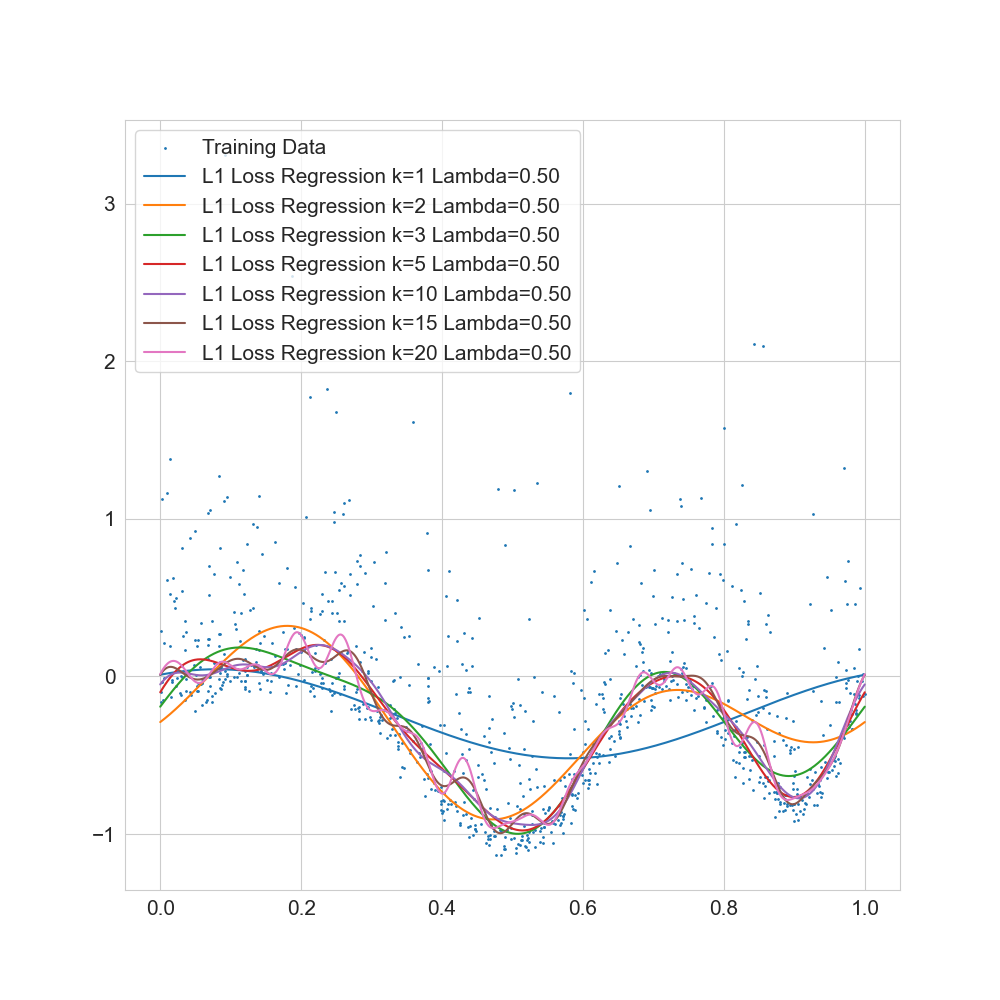
\includegraphics{../figures/normalized_l1_regression_all_k_lambda_0.50.png}
        \caption{L1 Loss Regression for all $k$ using Nomalized Basis Functions}
    \end{subfigure}%
    \begin{subfigure}[b]{.5\textwidth}
        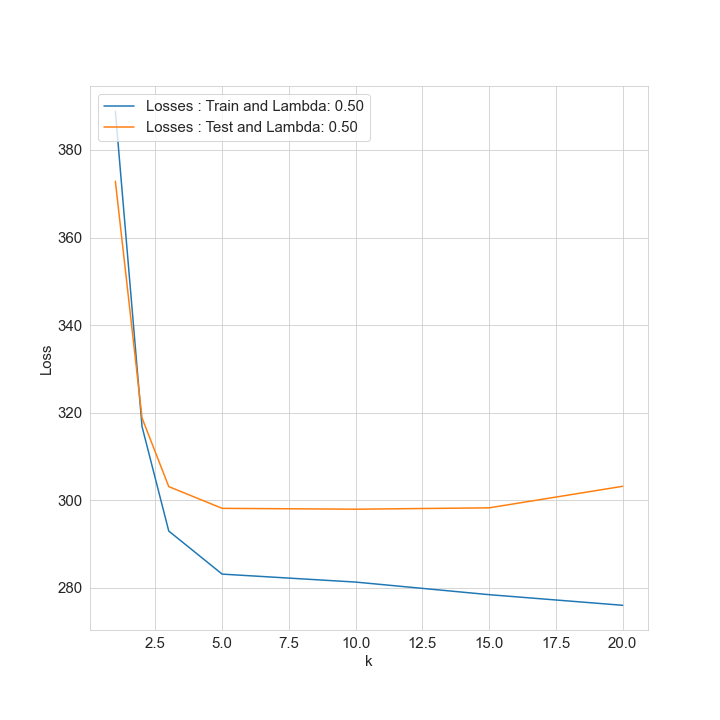
\includegraphics{../figures/normalized_l1_losses_for_k_lambda_0.50.png}
        \caption{Training and Test Loss for L1 Loss Regression using Nomalized Baisis Functions}
    \end{subfigure}
    \caption{ Using normalized basis functions. }
   \end{figure}
    \FloatBarrier



\item \textbf{(2 points)} We now consider a modified problem where instead of penalizing the weights one directly penalises the gradient of the estimated function $f_w(x) = \langle w, \Psi(x)\rangle$:

\begin{equation}
        w^k = argmin_{w \in \mathbb{R}^2k} \frac{1}{n} \sum_{i=1}^n (Y_i  - f_w(X_i))^2 + \lambda \Omega(f_w)
\end{equation}

where $\Omega(f)$ is defined in part d. Show that when using the normalized Fourier basis $\Psi_i$ without the constant 
function $\Psi_0$ the above optimization problem is equivalent to ridge regression that is $\Omega(f_w) = ||w||^2$.

Zip all plots (.png), scripts (.py), test (.pdf). In addition to the functions mentioned above, there 
should be scripts to reproduce all the results you submit (plots, losses).

\end{enumerate}

\bibliography{sample-handout}
\bibliographystyle{plainnat}
\end{document}
